\documentclass[12pt]{article}
\usepackage[letterpaper,top=2cm,bottom=2cm,left=1.8cm,right=1.8cm,marginparwidth=1.75cm]{geometry}
\usepackage{graphicx} % Required for inserting images
\usepackage[english]{babel}
\usepackage[T1]{fontenc}
\usepackage{listings}
\usepackage{float}
%\%\%usepackage[nomarkers]{endfloat}
\usepackage{color}
\usepackage{xcolor}
\usepackage{tikzducks}
\usepackage{lipsum}
\usepackage{amsmath,amsthm}
\usepackage{amssymb}
\usepackage{isomath}
\usepackage{changepage}
\usepackage{algorithm}
\usepackage{algpseudocode}
\usepackage{colortbl}
\usepackage{caption} 
\usepackage{array}
\usepackage{multicol} % Pour les colonnes
\usepackage[hidelinks]{hyperref}
\usepackage{csquotes}
\usepackage{tikz}
\usepackage[
backend=biber,
style=numeric
]{biblatex}
\addbibresource{biblio.bib}


\newcommand{\K}{\mathbb{K}}
\newcommand{\N}{\mathbb{N}}
\newcommand{\C}{\mathbb{C}}
\newcommand{\R}{\mathbb{R}}
\newcommand{\Rd}{\mathbb{R}^d}
\newcommand{\I}{\mathbf{I}}
\newcommand{\dcrochetg}{[\![}
\newcommand{\dcrochetd}{]\!]}
\newcommand\independent{\protect\mathpalette{\protect\independenT}{\perp}}
\def\independenT#1#2{\mathrel{\rlap{$#1#2$}\mkern2mu{#1#2}}}

%Gary's stuff 
\newtheorem{thm1}{Théorème}[section]
\newtheorem{lemme1}[thm1]{Lemme}
\newtheorem{prop1}[thm1]{Proposition}
\newtheorem*{rmq1}{Remarque}
\newtheorem*{exemple1}{Exemple}
\newtheorem*{defin1}{Définition}
%End of Gary's stuff


\begin{document}
\title{How to classify responses to adversity: resilience and vulnerability as deviations from the average}
\author{Garance Malnoë under the supervision of Jan Höltge}
\date{May - July 2025}

\pagenumbering{gobble}
\maketitle
\tableofcontents
\clearpage
\pagenumbering{arabic}
\section{Introduction / Main Contribution}

The main contribution of this work is the introduction of new classification methods for analysing individual responses to adversity in the context of resilience research. These methods offer a shift in perspective by conceptualising resilience and vulnerability not as dominant response types, but as deviations from the norm. We propose to identify resilient and vulnerable individuals as those whose outcomes are notably better or worse, respectively, than the typical response to a given level of adversity.\\
\\
With this framework, we provide tools to classify individuals into three groups: an average or normative group, consisting of individuals whose response is close to the expected or mean response for their level of adversity; a resilient group, whose outcomes are better than expected; and a vulnerable group, whose outcomes are worse. These classifications are based on the residuals obtained from a regression of outcome on adversity.\\
\\
Our approach is designed to be flexible and generalizable: all methods can be implemented using open-source standard statistical tools in R, and they are applicable across a wide range of settings and resilience constructs.\\
\\
In the context of cross-sectional data, we present different approaches to define thresholds of deviation, including approaches based on quantiles, confidence intervals, prediction intervals, credibility intervals, standard deviation, and the k-means algorithm.\\
\\
We extend this framework to longitudinal data using a Bayesian mixed-effects model with spike-and-slab priors for random effect selection. This allows us to identify individuals whose response systematically deviates from the average pattern, again classifying them as resilient, vulnerable, or average depending on the direction and significance of the deviation.\\
\\
This document will be separated into two parts. First, we introduce multiple cross-sectional classification methods based on residuals from a linear regression between an adversity variable and an outcome variable, where, to ensure robustness, we systematically identified and excluded from the fitting overly influential individuals using standard influence diagnostics. We then present the results of these classification methods on a real-world dataset and assess the relevance of each method by evaluating how well the resulting classification supports predictive modelling. Second, we extend the framework to longitudinal data by modelling the residuals of multiple regressions over time with a mixed-effects approach and present the spike-and-slab methodology to detect persistent deviations from the normative response. Then, we illustrate this method on another real-world dataset. Both illustrations are fully implemented with open-source tools in R.

\section{Cross-sectional Analysis}
\subsection{Methods}
\subsubsection{Overview}
In the cross-sectional setting, our objective is to identify individuals whose outcomes deviate from the average response to adversity evaluated at a single point in time.\\
\\
To do so, we begin by fitting a linear regression model in which an outcome variable (e.g., a psychological functioning score) is regressed on an adversity variable (e.g., a cumulative adversity index). The residuals from this model capture individual deviations from the expected response, given the observed level of adversity.\\
\\
To ensure that the fitted model is not unduly influenced by some individuals, we use influence diagnostics, specifically Cook's distance, to identify overly influential individuals. These individuals are excluded from the model fitting, but we still compute their residuals from the fitted model for completeness.\\
\\
Finally, individuals are classified into three groups (resilient, average, vulnerable) based on the distribution of residuals, using one of several methods introduced in the classification methods definition section.

\subsubsection{Residualisation}
The first step of the method consists of fitting a linear regression model where an outcome variable is regressed on an adversity variable. This residual-based approach to measuring resilience is commonly used and validated in the literature \cite{validity_of_residual_approach}. Formally, the model is written as:
\[
\vectorsym{y} = \matrixsym{X}\vectorsym{\hat\beta} + \vectorsym{\epsilon}\\
\]
Where \( \vectorsym{y} \in \mathbb{R}^n \) is the vector of outcomes, \( \matrixsym{X} \in \mathcal{M}_{n,2}(\R) \) is the design matrix with a column of ones and a column containing the adversity scores, \( \vectorsym{\hat\beta} \in \mathbb{R}^2 \) is the vector containing the intercept and slope coefficients, and \( \vectorsym{\epsilon} \in \mathbb{R}^n \) is the vector containing the residuals. The residual for each individual corresponds to the difference between their observed outcome and the predicted outcome given their level of adversity.\\
\\
It's worth noting that the direction of the association between adversity and outcome varies depending on the choice of variables. Thus, the sign of the residuals must be interpreted in context: when a higher outcome score means better functioning, a positive residual reflects a better outcome whereas when a higher outcome means worse functining, a positive residual reflects a worse outcome, as you can see in Figure \ref{fig:interpretation_sign_residuals}.
\begin{figure}[H]
    \centering
    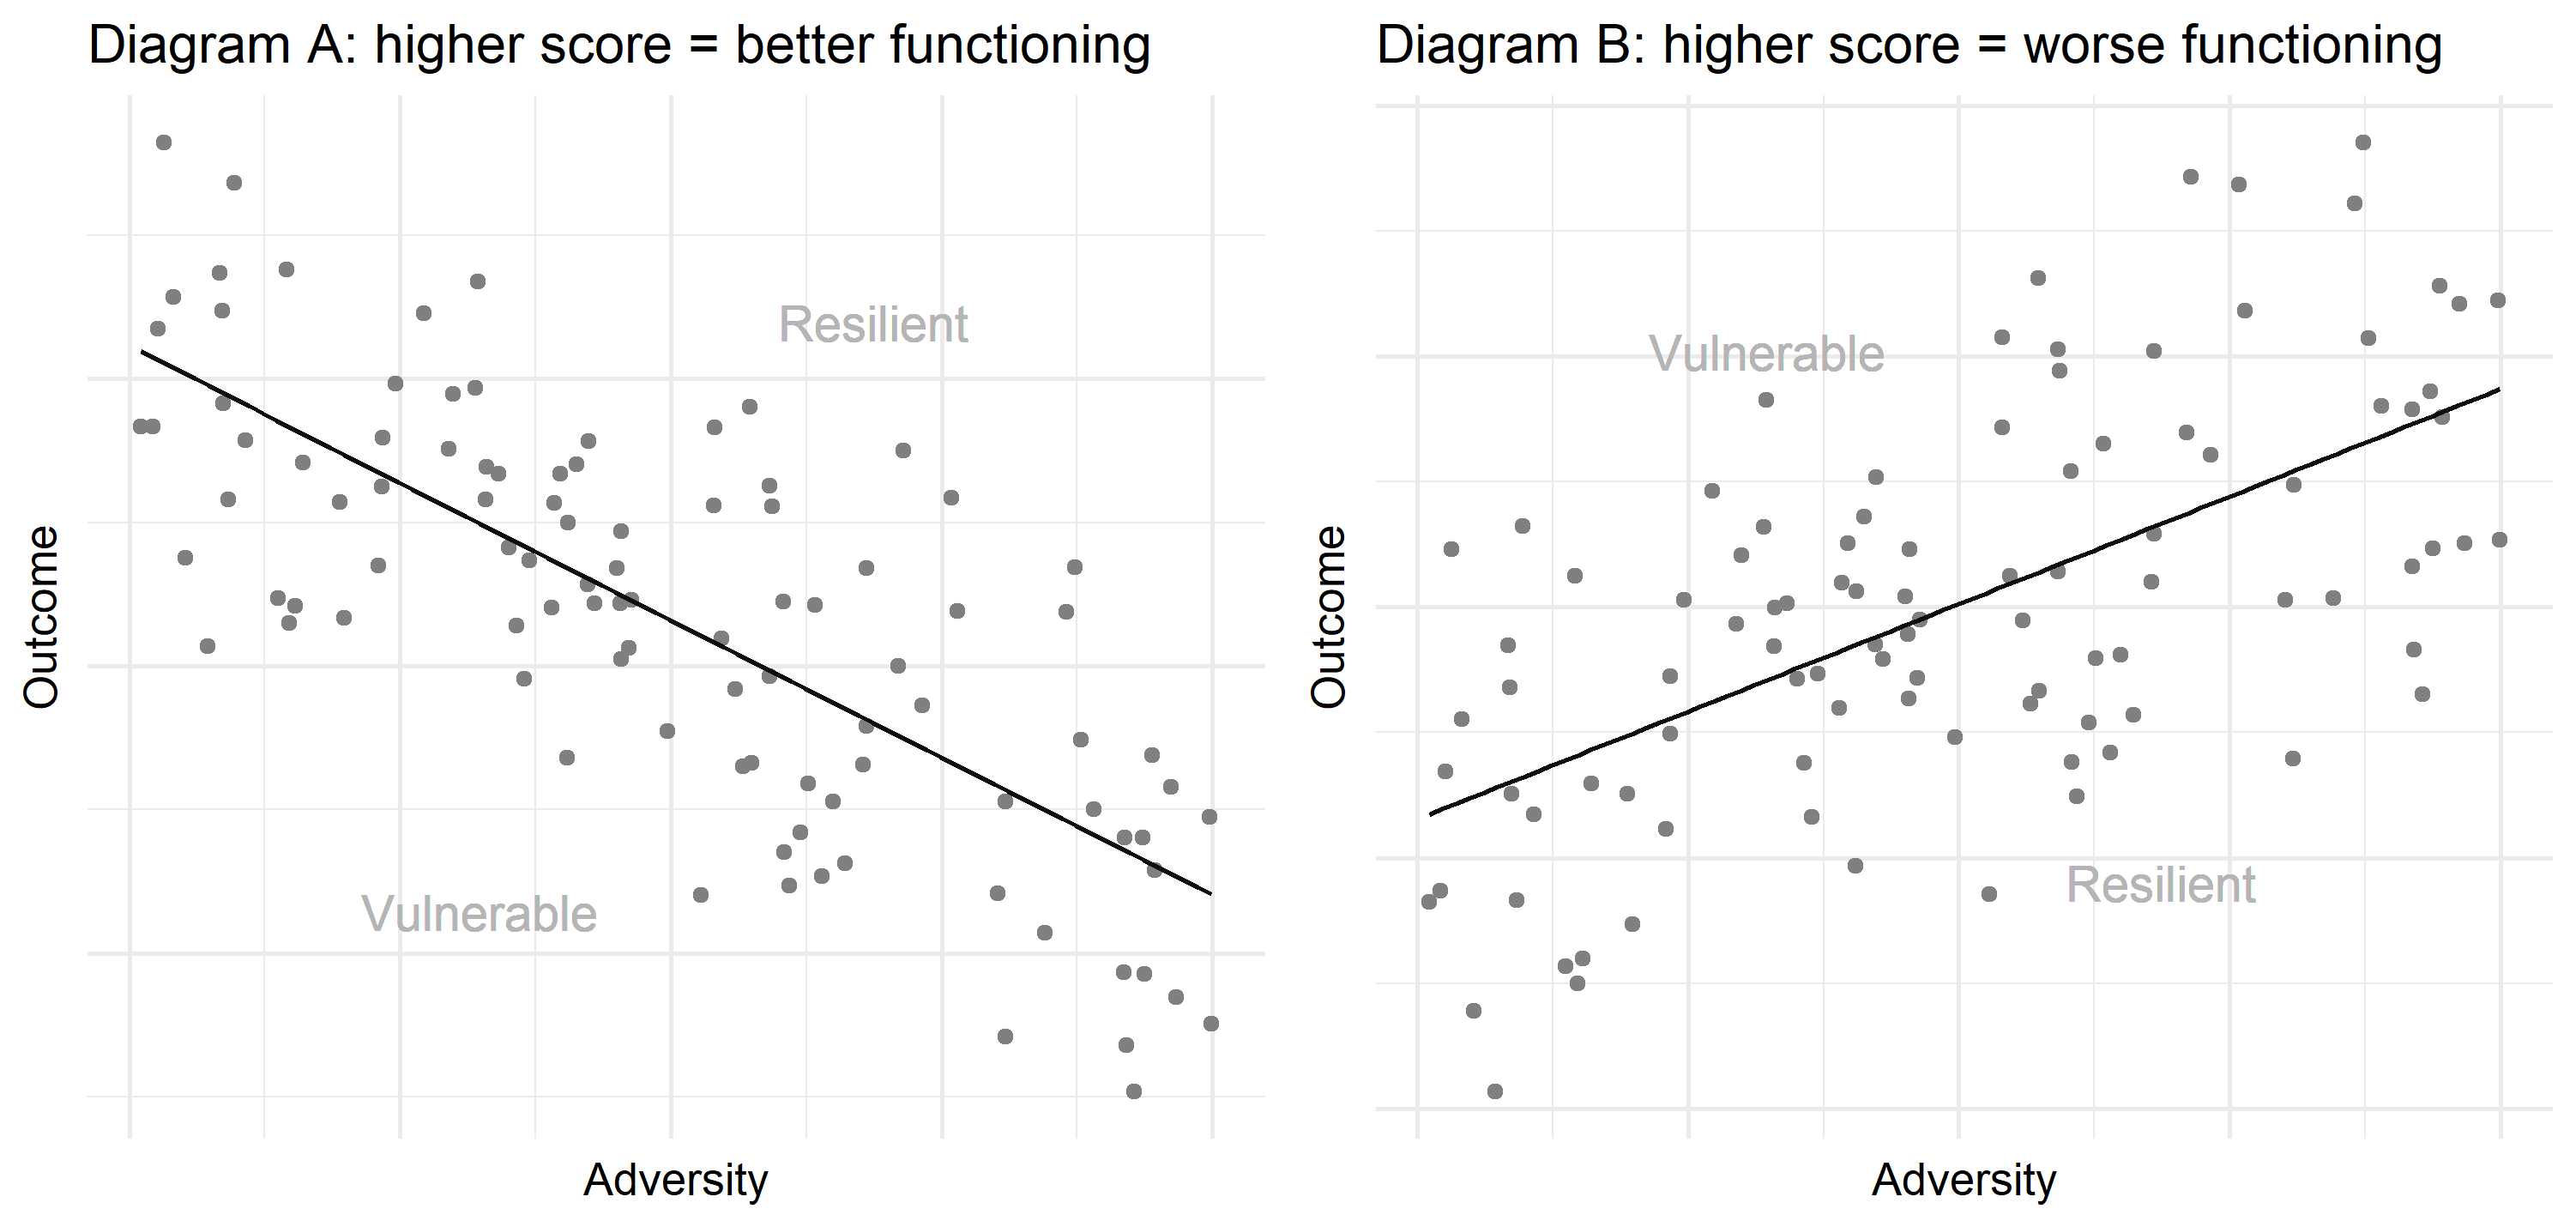
\includegraphics[width=18cm]{Pictures/Diagram_placement_vulnerable_resilient.png}
    \caption{Diagrams explaining the meaning of a residual depending on its sign and the direction of the regression}
    \label{fig:interpretation_sign_residuals}
\end{figure}
\subsubsection{Influence statistics}
To ensure robustness in the estimation of the regression model, we apply influence diagnostics to identify and exclude overly influential individuals. Following the recommendations of \cite{influencial_stat_residuals}, we inspect each individual's Cook's distance, which quantifies the impact of removing that individual on the estimated regression coefficients. Cook's distance is defined as:
\[
D_j = \frac{(\boldsymbol{\hat\beta} - \boldsymbol{\hat\beta}_{(j)})^\top \mathbf{X}^\top \mathbf{X} (\boldsymbol{\hat\beta} - \boldsymbol{\hat\beta}_{(j)})}{p s^2}\\
\]
where \( \boldsymbol{\hat\beta} \) is the vector of estimated coefficients using the full dataset, \( \boldsymbol{\hat\beta}_{(j)} \) is the coefficient vector estimated without the $j^{th}$ individual, \( \mathbf{X} \) is the design matrix, \( p \) is the number of parameters in the model (i.e., the rank of \( \mathbf{X} \)), and \( s^2 \) is the mean squared error of the full model.\\
\\
Individuals with a Cook’s distance strictly greater than \( 4/n \), where \( n \) is the sample size, are considered overly influential and are excluded from the regression fitting. However, we still compute their residuals from the fitted model, so that all individuals are retained in the classification step that follows. 

\subsubsection{Classification methods definition}
Using the residuals obtained from the residualisation, we propose several approaches to define class membership between resilient, normative and vulnerable:

\begin{itemize}
\item \textbf{Naïve approach:} Individuals with a non-null residual are classified as resilient or vulnerable depending on the sign of the residual and the relationship between the adversity and the outcome; individuals with a null residual are classified as average.

\item \textbf{Confidence and prediction interval-based classification:}  
Individuals are classified based on how their observed outcome compares to the expected interval under the regression model. Specifically, we use either confidence intervals (intervals for the mean predicted outcome) or prediction intervals (intervals for a new individual outcome). An individual is classified as average if their outcome falls within the chosen interval. Otherwise, they are classified as resilient or vulnerable, depending on the sign of their residual.\\
\\
Formally, let \( x_0 \in \mathbb{R}^p \) be the design vector for an individual (i.e., a vector with a one for the intercept and the individual's adversity score). The corresponding prediction is:
\[
\hat y_0 = x_0^\top \hat{\boldsymbol{\beta}}.\\
\]
The \( 100(1 - \alpha)\% \) confidence interval for \(\hat y_0\) is given by:
\[
\left[ \hat y_0 \; \pm \; t_{n-p,\,1 - \frac{\alpha}{2}} \cdot SE_{\text{mean}}(x_0) \right],\\
\]
where
\[
SE_{\text{mean}}(x_0) = \hat{\sigma} \cdot \sqrt{x_0^\top (\mathbf{X}^\top \mathbf{X})^{-1} x_0},
\]
\( \hat{\sigma}^2 \) is the estimated residual variance, and \( t_{n-p,\,1 - \frac{\alpha}{2}} \) is the quantile of the Student distribution with \( n - p \) degrees of freedom.\\
\\
The \( 100(1 - \alpha)\% \) prediction interval for a new observation at \( x_0 \) is:
\[
\left[ \hat y_0 \; \pm \; t_{n-p,\,1 - \frac{\alpha}{2}} \cdot SE_{\text{pred}}(x_0) \right],
\]
where
\[
SE_{\text{pred}}(x_0) = \hat{\sigma} \cdot \sqrt{1 + x_0^\top (\mathbf{X}^\top \mathbf{X})^{-1} x_0}.\\
\]
The prediction interval is wider than the confidence interval, as it accounts for both the uncertainty in estimating the mean and the variability of individual outcomes \cite{confidence_and_prediction_intervals}.

\item \textbf{Credibility interval-based classification:}  
Instead of the original linear regression model, we fit a Bayesian linear regression model using the same sample (i.e., excluding influential individuals). We use the \texttt{stan\_glm()} function from the \texttt{rstanarm} package (version~2.32.1) to estimate the relationship between the outcome variable and the adversity variable, using the default weakly informative priors as implemented in \texttt{rstanarm}.

After fitting the model, we use the \texttt{posterior\_linpred()} function to generate \(S=1000 \) draws from the posterior predictive distribution of the expected outcome for each individual, conditional on their observed adversity level. Specifically, for each \( x_j \), we compute:

\[
\hat{y}_j^{(s)} = \beta_0^{(s)} + \beta_1^{(s)} x_j \quad \text{for } s = 1, \ldots, S\, ,
\]

where \( \hat{y}_j^{(s)} \) is the predicted mean outcome from the \( s \)-th posterior draw. This yields a posterior distribution of expected outcomes for each individual.

To construct individual-level credibility intervals, we compute the empirical \( \alpha/2 \) and \( 1 - \alpha/2 \) quantiles of the \( \hat{y}_j^{(s)} \) values. Individuals whose observed outcome \( y_j \) falls within their corresponding \( 100(1 - \alpha)\% \) posterior credibility interval are classified as average. Those with outcomes outside the interval are classified as either resilient or vulnerable, depending on the direction of the deviation.
\item \textbf{Quantile-based thresholds:} Individuals are classified based on the empirical distribution of residuals. Those with residuals below the \( n\% \) quantile or above the \( (100-n)\% \) quantile are identified as atypical (resilient or vulnerable). Individuals with residuals within this central range are classified as average.

  \item \textbf{Standard deviation-based thresholds using adversity levels:} For each adversity score interval (e.g. 5 by 5 or levels associated with the variable), the standard deviation of the residuals of all individuals belonging to this level is computed. Individuals whose residuals deviate by more than 0.5, 1 or 2 times (or another multiple) the standard deviation of the level they belong to are then considered atypical (resilient or vulnerable), and the ones inside the interval are considered average.
  \item \textbf{K-means classification:} Application of the k-means algorithm on the residual values with 3 clusters and random start-points. The group with the intermediary mean residual value is considered the average group. Depending on the direction of the relationship between the adversity and the outcome, the two other groups are the resilient and vulnerable.
\end{itemize}
Those different methods allow for different sizes of the average group, but also different shapes, as you can see in the illustrative example.

\subsection{Illustrative Example: RYSE Project}
\subsubsection{Data and Variables}
For our illustrative example, we used data from the Resilient Youth in Stressed Environments (RYSE) project \cite{site_RYSE}, first reported in \cite{first_RYSE}. The project aimed to investigate the multisystemic factors and processes underpinning resilience in adolescents (aged 14–24) living in communities dependent on the oil and gas industries in Canada and South Africa. During data collection waves in 2018, 2019, and 2020, these communities experienced severe economic recessions, leading to high rates of unemployment and family tension, as well as increased levels of anxiety and depression among adolescents.\\
\\
For this analysis, we focused exclusively on data collected in 2018 and restricted our sample to participants from the South African site, due to the cultural differences between the two study locations. We retained individuals who had non-missing values for the SES or WES adversity variables and a non-missing score on the BDI-II depression scale, and who had at most 30\% of missing responses across all variables. Missing values were imputed using the \texttt{missForest} function from the \texttt{missForest} package (version~1.4); age and sex did not have to be unimputed.\\
\\
After preprocessing, the final dataset included \(N=423 \) participants. The variables used in the analysis are described in Table~\ref{table:RYSE_variables}.\\
\\
For this illustrative example, we used either the School Engagement Scale (SES) or the Work Engagement Scale (WES) as the outcome variable, depending on each participant's context. Specifically, if an individual had both SES and WES scores available, we selected SES for those in grades 9 to 12 and WES otherwise. To ensure comparability between these two scales, which have different ranges and distributions, we linearly rescaled their values to a common 0–100 range and combined them into a single “Engagement” variable used as the outcome. The Beck Depression Inventory-II (BDI-II) score was used as the adversity variable.

\begin{table}[H]
\centering
\rowcolors{2}{gray!20}{white} % Gris sur une ligne sur deux
{\small
\begin{tabular}{>{\centering\arraybackslash}p{1.2cm}
                >{\centering\arraybackslash}p{4.3cm}
                >{\centering\arraybackslash}p{8cm}
                >{\centering\arraybackslash}p{2.5cm}}
\hline
\textbf{Name} & \textbf{Values (discrete)} & \textbf{Description} &  \textbf{Type} \\
\hline
BDI-II & 0-63 & Beck's Depression Inventory (measurement of depression's severity)& Adversity\\
WES & 9-63 & Work Engagement Scale& Outcome\\
SES & 33-165 & School Engagement Scale & Outcome\\
Age & 14-24 & Age of the participant at the moment of the measurement & Explanatory\\
Sex & Female, male, other& Sex of the participant& Explanatory\\
SF-15 & 0-100 & Short-Form health survey 15& Explanatory\\
CPTS & 0-80 & Childhood Post-traumatic stress scale& Explanatory\\
CYRM & 28-140 & Child and Youth Resilience Measure& Explanatory\\
PoNS & 10-40 & Perception of Neighborhood Scale& Explanatory\\
FAS & 0-10 & Family Adversity Scale& Explanatory\\
BCE & 0-10 & Benevolent Childhood Experiences & Explanatory\\
\hline
\end{tabular}
}
\caption{Variables used from the RYSE project}
\label{table:RYSE_variables}
\end{table}

\subsubsection{Software}
All models were implemented in \texttt{R} (version~4.4.3) using the packages \texttt{dplyr} (version~1.1.4), \texttt{missForest} (version~1.4), \texttt{haven} (version~2.5.5) to read the data, \texttt{olsrr} (version~0.6.1) for the influence statistics and \texttt{rstanarm} (version~2.32.1).

\subsubsection{Residualization results}
Twenty-five individuals were identified as overly influential based on Cook's distance and were excluded from the adjusted model. Figure~\ref{fig:adjusted regression} presents the results of both the unadjusted and adjusted linear regressions, with overly influential individuals marked as filled points. While the models yield broadly similar results, the adjusted model shows a smaller slope coefficient (in absolute value) than the unadjusted one, indicating a slightly attenuated relationship after excluding influential observations.\\
\\
Higher scores on the Engagement variable indicate better functioning, whereas higher BDI-II scores correspond to more severe depression. Consequently, the observed negative association between the adversity and the outcome implies that individuals with positive residuals are functioning better than expected given their BDI-II score, while those with negative residuals are functioning worse than expected.

\begin{figure}
    \centering
    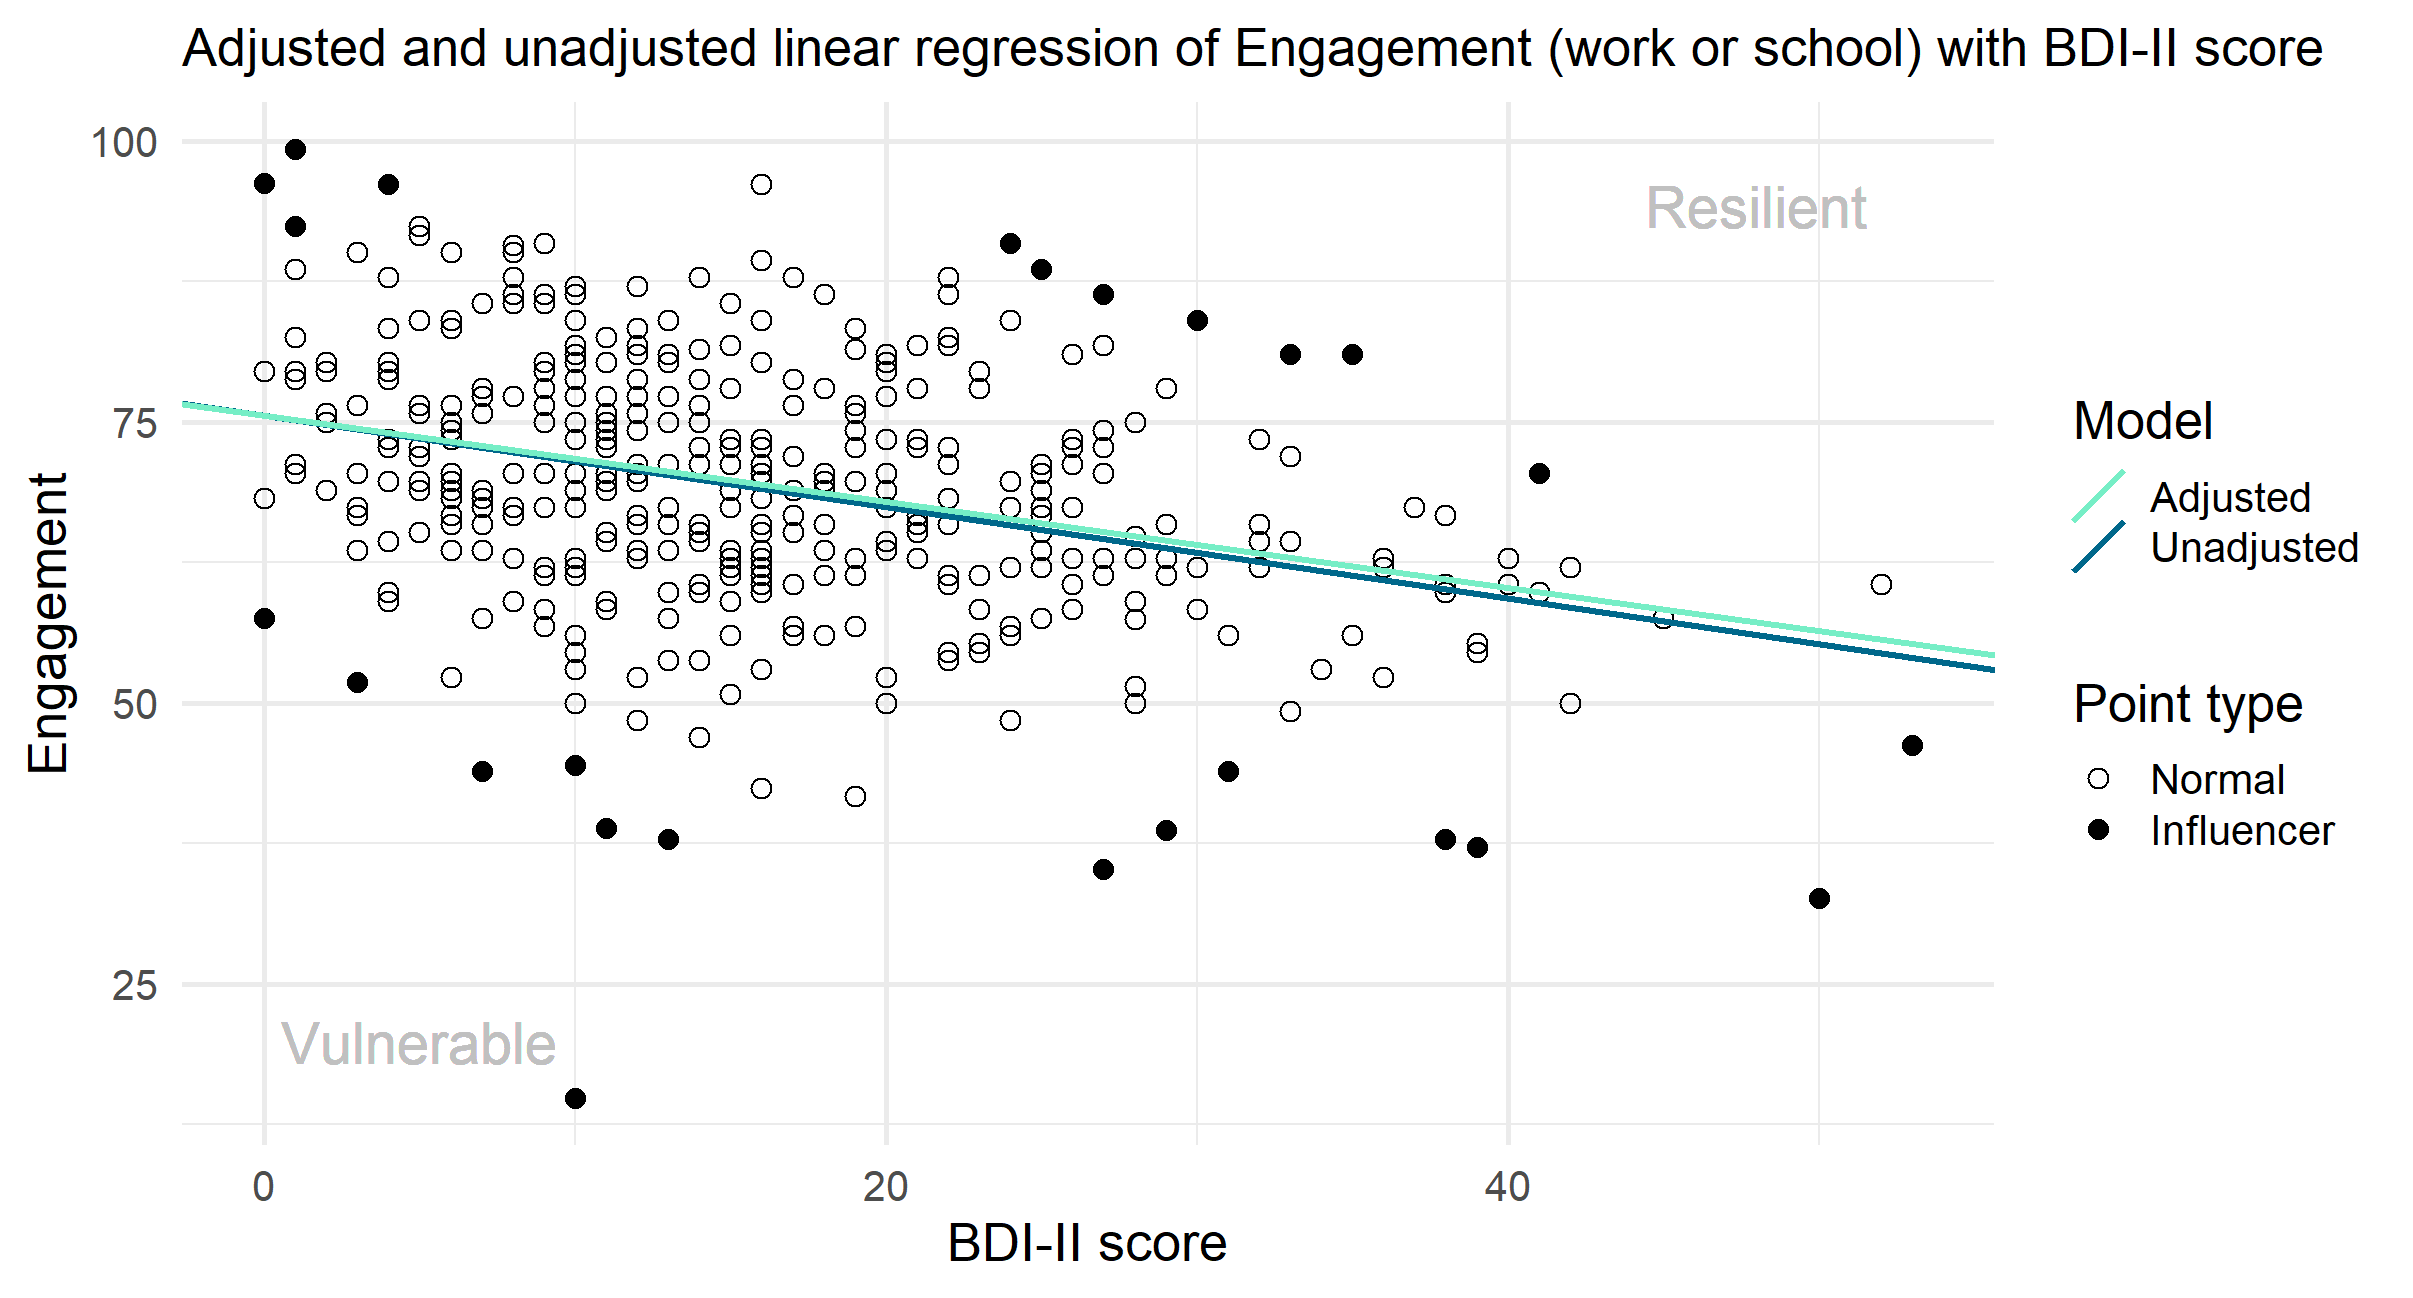
\includegraphics[width=19cm]{Pictures/adjusted_regression.png}
    \caption{Adjusted and unadjusted linear regressions of engagement (work or school) with BDI-II score}
    \label{fig:adjusted regression}
\end{figure}

\subsubsection{Group results by method}
We applied each classification method to the residuals from the adjusted linear regression and computed the resulting group memberships across all individuals.

\subsubsection*{Naive approach}
As shown in Table~\ref{table:size-naive}, the naive classification method results in an extreme case where no individuals are classified as average, all individuals are assigned either to the resilient or vulnerable group. Figure \ref{fig:classification_naive} illustrates that this method imposes a strict split at zero, without accounting for the variability or uncertainty of the residuals. Even individuals with residuals very close to zero are considered atypical. This method is therefore intended more as a baseline comparison than as a realistic classification approach.

\begin{table}[H]
\centering
\rowcolors{2}{gray!20}{white} % Gris sur une ligne sur deux
{\small
\begin{tabular}{>{\centering\arraybackslash}p{3cm}
                >{\centering\arraybackslash}p{3cm}
                >{\centering\arraybackslash}p{3cm}}
\hline
\textbf{Resilient size} & \textbf{Average size} & \textbf{Vulnerable size} \\
\hline
210 & 0 & 213 \\
\hline
\end{tabular}
}
\caption{Group size with the naive approach}
\label{table:size-naive}
\end{table}

\begin{figure}
    \centering
    
\includegraphics[width=18cm]{Pictures/Visualization_groups/naive.png}
    \caption{Classification obtained with the naive approach}
    \label{fig:classification_naive}
\end{figure}

\subsubsection*{Confidence and prediction interval-based classification}
As shown in Table~\ref{table:size-confidence_pred} and Figure~\ref{fig:conf_pred-classification}, prediction intervals produce wider intervals and thus larger average groups compared to confidence intervals. The 3 values tested for prediction intervals ($50,60$ and $75$\%) resulted in a dominant average group, but the two confidence intervals tested ($99$ and $90$\%) did not result in a dominant average group. As expected, decreasing the confidence or prediction level (i.e., using a smaller \(1-\alpha \)) results in narrower intervals and, consequently, smaller average groups. \\
\\
An important distinction is that, in our example, confidence intervals vary much more in width across levels of adversity than prediction intervals. This is because, in our data, the leverage term \( x_0^\top (\mathbf{X}^\top \mathbf{X})^{-1} x_0 \) remains below $0.05$, leading to a wider range of variation for the confidence interval widths:
\[
0.05019 \leq \text{SE}_{\text{mean}}(x_0) \leq 0.20852,
\]
compared to the prediction interval widths:
\[
1.001 \leq \text{SE}_{\text{pred}}(x_0) \leq 1.022.
\]
As a result, the prediction intervals appear almost uniform across the range of adversity, while the confidence intervals are more sensitive to the adversity level of the individual.


\begin{table}[H]
\centering
\rowcolors{2}{gray!20}{white} % Gris sur une ligne sur deux
{\small
\begin{tabular}{>{\centering\arraybackslash}p{5cm}
                >{\centering\arraybackslash}p{3cm}
                >{\centering\arraybackslash}p{3cm}
                >{\centering\arraybackslash}p{3cm}}
\hline
\textbf{Detail}&\textbf{Resilient size} & \textbf{Average size} & \textbf{Vulnerable size} \\
\hline
Prediction interval 75\% &63&300 &60 \\
Prediction interval 60\% & 93&240 &90\\
Prediction interval 50\% & 105&208 &110\\
Confidence interval 99\% &181 & 53&189\\
Confidence interval 90\%&190 &37 &196\\
\hline
\end{tabular}
}
\caption{Group size with the confidence and prediction intervals approach}
\label{table:size-confidence_pred}
\end{table}
\begin{figure}
    \centering
    
\includegraphics[width=18cm]{Pictures/Visualization_groups/conf_pred.png}
    \caption{Classification obtained with the confidence and prediction intervals approach}
    \label{fig:conf_pred-classification}
\end{figure}

\subsubsection*{Credibility interval-based classification}
As shown in Figure~\ref{fig:credibility-classification} and Table~\ref{table:size-credibility}, credibility intervals tend to be very narrow, resulting in small average groups, even when using wide intervals such as the 99.9\% credibility level. In practice, the class size produced by credibility intervals closely resembles those obtained from confidence intervals of the same level.\\
\\
As with confidence intervals, the width of credibility intervals varies with the level of adversity, since they reflect posterior uncertainty around the expected outcome for each individual.

\begin{table}[H]
\centering
\rowcolors{2}{gray!20}{white} % Gris sur une ligne sur deux
{\small
\begin{tabular}{>{\centering\arraybackslash}p{4cm}
                >{\centering\arraybackslash}p{3cm}
                >{\centering\arraybackslash}p{3cm}
                >{\centering\arraybackslash}p{3cm}}
\hline
\textbf{Detail}&\textbf{Resilient size} & \textbf{Average size} & \textbf{Vulnerable size} \\
\hline
Credibility interval 99.9\% & 176& 67 & 180 \\
Credibility interval 99\% & 188 & 52 & 183 \\
Credibility interval 95\% & 195 & 41&187 \\
Credibility interval 90\% & 198& 34& 191\\
Credibility interval 75\% & 202 & 25 & 196 \\
Credibility interval 50\% & 209 & 13 & 201 \\
\hline
\end{tabular}
}
\caption{Group size with the credibility intervals approach}
\label{table:size-credibility}
\end{table}
\begin{figure}
    \centering
    
\includegraphics[width=18cm]{Pictures/Visualization_groups/cred.png}
    \caption{Classification obtained with the credibility intervals approach}
    \label{fig:credibility-classification}
\end{figure}

\subsubsection*{Quantile-based thresholds}
In this approach, quantile thresholds were computed using only individuals not identified as overly influential, but the resulting classifications were applied to the full sample. As shown in Table~\ref{table:size-quantiles}, the quantile-based method yields approximately symmetrical group sizes by construction, with typically fewer than four individuals separating the resilient and vulnerable groups.\\
\\
The size of the average group depends directly on the chosen quantile level \( n\% \). For example, setting \( n = 5\% \) to \( 30\% \) results in a dominant average group. However, beyond \(n=35\% \), the average group becomes smaller than the two atypical groups combined.\\
\\
This method is particularly useful when a predefined proportion of the population is intended to be classified as atypical or normative, offering direct control over group sizes.

\begin{table}[H]
\centering
\rowcolors{2}{gray!20}{white} % Gris sur une ligne sur deux
{\small
\begin{tabular}{>{\centering\arraybackslash}p{4cm}
                >{\centering\arraybackslash}p{3cm}
                >{\centering\arraybackslash}p{3cm}
                >{\centering\arraybackslash}p{3cm}}
\hline
\textbf{Detail}&\textbf{Resilient size} & \textbf{Average size} & \textbf{Vulnerable size} \\
\hline
5\% & 30& 359& 34\\
10\% & 50& 320& 53\\
15\% & 71 & 279& 73\\
20\% &  92& 237 & 94\\
25\% & 111& 198& 114\\
30\% & 131& 158& 134\\
35\% & 150& 120& 153\\
\hline
\end{tabular}
}
\caption{Group size with the approach}
\label{table:size-quantiles}
\end{table}

\subsubsection*{Standard deviation based thresholds with adversity levels}
The standard deviation-based approach was applied using standardised cutoffs for BDI-II scores: 0–13 (minimal depression), 14–19 (mild), 20–28 (moderate), and 29–63 (severe).\\
\\
Like for the quantiles, we used the individuals that were marked as not overly influential to compute the standard deviation of each bins, but we applied the classification to all individuals.\\
\\
As shown in Table~\ref{table:size-sd} and Figure~\ref{fig:sd-classification}, this approach can produce either very large or very small average groups depending on the chosen threshold. For example, using a threshold of 0.5 SD around the prediction results in approximately 35\% of individuals being classified as average, whereas a 2 SD threshold yields an average group comprising around 91\% of the sample.\\
\\
This method also allows the width of the average band to vary across adversity levels, as the standard deviation is computed within each category. In the present case, this provides an additional layer of flexibility, with the classification adapting to the variability present within each adversity group.

\begin{table}[H]
\centering
\rowcolors{2}{gray!20}{white} % Gris sur une ligne sur deux
{\small
\begin{tabular}{>{\centering\arraybackslash}p{4cm}
                >{\centering\arraybackslash}p{3cm}
                >{\centering\arraybackslash}p{3cm}
                >{\centering\arraybackslash}p{3cm}}
\hline
\textbf{Detail (multiplication)}&\textbf{Resilient size} & \textbf{Average size} & \textbf{Vulnerable size} \\
\hline
2SD &  15& 387& 21\\
1SD &  80& 265& 78\\
0.5SD &  131&151&141\\
\hline
\end{tabular}
}
\caption{Group size with the standard deviation approach}
\label{table:size-sd}
\end{table}
\begin{figure}
    \centering
    
\includegraphics[width=18cm]{Pictures/Visualization_groups/sd.png}
    \caption{Classification obtained with the standard deviation approach}
    \label{fig:sd-classification}
\end{figure}

\subsubsection*{K-means classification}
Again, for this approach, we only used the individuals identified as not overly influential to construct the k-means clusters. The remaining individuals were assigned to the cluster whose centre they were closest to.\\
\\
As shown in Figure~\ref{fig:kmeans-classification} and Table~\ref{table:size-kmeans}, the classification produced by the k-means-based approach is not symmetrical: the resilient group is smaller than the vulnerable group, and the average and vulnerable groups are of equal size. This reflects the data-driven nature of the method, which does not impose balanced group sizes or fixed thresholds, but instead discovers clusters based on the structure of the residual distribution.\\
\\
An advantage of this approach is that, despite relying solely on the data, it still identifies a central group composed of individuals with small positive and small negative residuals, corresponding well to the notion of an average or normative response. In contrast, unsupervised methods could, in principle, produce less interpretable groupings (e.g., two clusters of positive residuals and one of negative), but this was not the case here. However, the fact that the vulnerable and average groups are equally large highlights the method’s sensitivity to distributional shape. In different datasets or residual distributions, a non-average group could become dominant, depending entirely on how the algorithm partitions the space.

\begin{table}[H]
\centering
\rowcolors{2}{gray!20}{white} % Gris sur une ligne sur deux
{\small
\begin{tabular}{>{\centering\arraybackslash}p{3cm}
                >{\centering\arraybackslash}p{3cm}
                >{\centering\arraybackslash}p{3cm}}
\hline
\textbf{Resilient size} & \textbf{Average size} & \textbf{Vulnerable size} \\
\hline
99& 162& 162\\
\hline
\end{tabular}
}
\caption{Group size with the k-means approach}
\label{table:size-kmeans}
\end{table}
\begin{figure}
    \centering
    
\includegraphics[width=18cm]{Pictures/Visualization_groups/k-means.png}
    \caption{Classification obtained with the k-means method}
    \label{fig:kmeans-classification}
\end{figure}


\subsubsection{Evaluation of predictive relevance}
$\cdots$

\section{Longitudinal Analysis}
\subsection{Methods}
The goal of this approach is to estimate which individuals consistently deviate from the mean trajectory over time, and therefore can be categorized as resilient or vulnerable depending on the sign of the deviation. As in the cross-sectional context, we use residualization to obtain individual-level measures of resilience. Specifically, at each time point, we fit a linear regression model in which an outcome variable is regressed on an adversity variable, and we use the residuals as the resilience indicator. Again, to ensure robustness, we exclude overly influential individuals from each regression based on Cook’s distance with the same $\frac{4}{n}$ threshold (where $n$ is the number of participants). This procedure is repeated independently at each time point.\\
\\
To model the resilience across time, we then fit a linear mixed-effects model to the residuals, with both fixed effects (capturing the mean trend over all individuals) and individual-level random intercepts. These random intercepts represent persistent deviations from the average trajectory (i.e., stable individual differences in resilience).\\
\\
To identify which individuals deviate significantly from the average trajectory, we apply the method introduced by \cite{spike_and_slab}, which relies on a Bayesian \textit{spike-and-slab} prior structure. This method estimates the probability that each individual's random effect differs from zero. Using this estimated probability, after setting a threshold, individuals below the threshold are classified as average, and individuals above the threshold are classified as resilient or vulnerable, depending on the sign of the deviation.\\
\\
The \textit{spike-and-slab} method models the random effect distribution as a mixture of two components:
\begin{itemize}
  \item a \textit{spike}, corresponding to a distribution concentrated at zero, representing individuals with no stable deviation;
  \item a \textit{slab}, a more diffuse distribution around zero, representing individuals with non-zero random effects.
\end{itemize}
An indicator variable determines, for each MCMC sample, whether an individual is assigned to the spike or slab component. The proportion of MCMC samples in the \textit{slab} is then used to approximate the posterior inclusion probability (PIP), i.e. the probability that the random effect deviates from zero, and that the individual consistently deviates from the mean and therefore is non-average. Individuals with PIPs below a set threshold are classified as average, while those exceeding the threshold are classified as either resilient or vulnerable, depending on the sign of their random effect.\\
\\
Note that it is necessary to specify the prior inclusion probability in the \textit{slab}, set between 0 and 1, which controls the selectivity of the model: a value of 0.5 reflects an absence of initial hypothesis on the presence of effects, while a higher value reflects a prior belief in the existence of non-zero effects.

\subsection{Illustrative Example: LORA Project}
\subsubsection{Data and Variables}
For this illustrative example, we used data from the Longitudinal Resilience Assessment (LORA) project, described in \cite{LORA}. The study was designed to investigate resilience mechanisms in response to everyday stress. The initial sample included \( N = 1{,}191 \) German-speaking adults aged 18 to 50 at baseline. Data was collected over a five-year period, with online questionnaires administered quarterly and in-depth assessments conducted every 18 months.\\
\\
For our analysis, we restricted the sample to \( N = 515 \) individuals who had completed all of the first \( T = 12 \) quarterly assessments. The Perceived Stress Scale (PSS) and the Daily Hassles questionnaire (DH) were used as adversity variables, and the General Health Questionnaire (GHQ) was used as the outcome variable. The scales and coding of these variables are described in Table~\ref{table:variables_lora}.


\begin{table}[H]
\centering
\rowcolors{2}{gray!20}{white}
{\small
\begin{tabular}{>{\centering\arraybackslash}p{1.5cm}
>{\centering\arraybackslash}p{4cm}
>{\centering\arraybackslash}p{9cm}
>{\centering\arraybackslash}p{2.5cm}}
\hline
\textbf{Name} & \textbf{Values (discretes)} & \textbf{Description} &  \textbf{Type} \\
\hline
PSS & 14–24 & Perceived Stress Scale & Adversity \\
DH & 14–24 & Daily Hassles& Adversity \\
GHQ & 0-84 & General Health Questionnaire & Outcome \\
\hline
\end{tabular}
}
\caption{Variables used from the LORA project}
\label{table:variables_lora}
\end{table}

\subsubsection{Software}
All models were implemented in \texttt{R} (version~4.4.3) using the packages \texttt{dplyr} (version~1.1.4), \texttt{rjags} (version~4.17), and \texttt{SSranef} (version~0.1.0). We fitted the models using the \texttt{ss\_ranef\_alpha()} function with its default settings, specifically:
\begin{itemize}
    \item 1,000 burn-in iterations,
    \item 1,000 sampling iterations for parameter estimation,
    \item 4 parallel MCMC chains,
    \item prior inclusion probabilities set to 0.5 for all individuals.
\end{itemize}


\subsubsection{Results}
The spike-and-slab method proved to be applicable and coherent in this longitudinal setting. Posterior inclusion probabilities (PIPs) were obtained for each individual, and group membership was assigned based on whether an individual’s PIP exceeded a chosen threshold. \\
\\
The posterior inclusion probabilities spanned a wide range. For the $GHQ\sim DH$ model, the PIPs ranged from 0.23 to 1.00, with a median of 0.52 and a mean of 0.58. For the $GHQ \sim PSS$ model, the range was 0.27 to 1.00, with a median of 0.44 and a mean of 0.55. These distributions confirm that most individuals were neither clearly average nor clearly non-average, and that the classification is sensitive to the choice of PIP threshold.\\
\\
Figures~\ref{fig:PIP_pss} and~\ref{fig:PIP_dh}, along with Tables~\ref{table:PIP_pss} and~\ref{table:PIP_dh}, show the evolution of group sizes as the PIP threshold increases for the $GHQ\sim PSS$ and $GHQ\sim DH$ models, respectively. In both models, increasing the PIP threshold leads to fewer individuals being classified as non-average, as expected.\\
\\
A small asymmetry between the resilient and vulnerable groups was observed in both models. For the $GHQ\sim PSS$  model, the vulnerable group was consistently slightly larger than the resilient group across all PIP thresholds. In contrast, for the $GHQ\sim DH$ model, the resilient group was slightly larger than the vulnerable group up to a threshold of 0.9, after which the trend reversed.\\
\\
These results confirm that the method is sensitive to the user-defined PIP threshold, while producing stable and interpretable classifications that are however slightly asymmetrical between the two non-average groups.

\begin{table}[H]
\centering
\rowcolors{2}{gray!20}{white}
{\small
\begin{tabular}{>{\centering\arraybackslash}p{1cm}
>{\centering\arraybackslash}p{4cm}
>{\centering\arraybackslash}p{4cm}
>{\centering\arraybackslash}p{4cm}}
\hline
PIP & Percentage atypical & Percentage resilient & Percentage vulnerable \\
\hline
0.50 & 45.44 & 21.55 & 23.88 \\ 
0.55 & 40.39 & 19.03 & 21.36 \\ 
0.60 & 36.70 & 16.50 & 20.19 \\ 
0.65 & 33.79 & 14.76 & 19.03 \\ 
0.70 & 31.07 & 13.79 & 17.28 \\ 
0.75 & 27.77 & 12.04 & 15.73 \\ 
0.80 & 24.47 & 11.07 & 13.40 \\ 
0.85 & 19.61 & 8.16 & 11.46 \\ 
0.90 & 16.70 & 6.99 & 9.71 \\ 
0.95 & 14.56 & 6.02 & 8.54 \\ 
1.00 & 6.60 & 1.94 & 4.66 \\ 
\hline
\end{tabular}
}
\caption{Proportions of individuals in each category depending on the chosen PIP threshold for GHQ $\sim$ PSS}
\label{table:PIP_pss}
\end{table}

\begin{figure}
    \centering
    
\includegraphics[width=18cm]{Pictures/longitudinal/pss.png}
    \caption{Proportions of individuals in each category depending on the chosen PIP threshold for GHQ $\sim$ PSS}
    \label{fig:PIP_pss}
\end{figure}

\begin{table}[H]
\centering
\rowcolors{2}{gray!20}{white}
{\small
\begin{tabular}{>{\centering\arraybackslash}p{1cm}
>{\centering\arraybackslash}p{4cm}
>{\centering\arraybackslash}p{4cm}
>{\centering\arraybackslash}p{4cm}}
\hline
PIP & Percentage atypical & Percentage resilient & Percentage vulnerable  \\
\hline
0.50 & 52.43 & 28.54 & 23.88 \\ 
0.55 & 47.77 & 26.60 & 21.17 \\ 
0.60 & 43.50 & 24.27 & 19.22 \\ 
0.65 & 40.58 & 23.11 & 17.48 \\ 
0.70 & 37.86 & 21.17 & 16.70 \\ 
0.75 & 35.73 & 19.81 & 15.92 \\ 
0.80 & 32.62 & 17.86 & 14.76 \\ 
0.85 & 28.74 & 14.95 & 13.79 \\ 
0.90 & 26.21 & 12.82 & 13.40 \\ 
0.95 & 20.58 & 9.51 & 11.07 \\ 
1.00 & 11.46 & 4.27 & 7.18 \\ 
\hline
\end{tabular}
}
\caption{Proportions of individuals in each category depending on the chosen PIP threshold for GHQ $\sim$ DH}
\label{table:PIP_dh}
\end{table}

\begin{figure}
    \centering
    
\includegraphics[width=18cm]{Pictures/longitudinal/dh.png}
    \caption{Proportions of individuals in each categories depending on the chosen PIP threshold for GHQ $\sim$ DH}
    \label{fig:PIP_dh}
\end{figure}


\newpage
\addcontentsline{toc}{section}{References}
\printbibliography

\end{document}
